% !TeX program = xelatex
% 由 教学课件/习题课模板/习题课模板.tex 复制并填充。
% 依据用户照片与独立数学核查；无例题、计算练习或评分。
% 教师用法：先停留在回忆提示，学生写出后再点击显示知识。
\documentclass[UTF8,10pt,aspectratio=169]{ctexbeamer}
\usepackage{amsmath,amssymb,tikz}
\usetikzlibrary{calc,arrows.meta,positioning}
\usepackage{newtxtext,newtxmath}
\usetheme{default}
\usecolortheme{default}
\usefonttheme{serif}
\setbeamertemplate{navigation symbols}{}
\setbeamertemplate{footline}[frame number]
\setbeamersize{text margin left=0.75cm,text margin right=0.75cm}
\setbeamerfont{normal text}{size=\large}
\setbeamerfont{frametitle}{size=\Large,series=\bfseries}
\setbeamerfont{itemize/enumerate body}{size=\large}
\setbeamerfont{itemize/enumerate subbody}{size=\large}
\AtBeginEnvironment{frame}{\large}
\setlength{\abovedisplayskip}{6pt}
\setlength{\belowdisplayskip}{6pt}
\definecolor{KnowledgeBlue}{RGB}{36,82,124}
\newcommand{\Recall}[1]{\par\noindent\textcolor{KnowledgeBlue}{\textbf{先回忆}\quad #1}\par\vspace{0.3cm}}
\newcommand{\Pitfall}[1]{\par\vspace{0.22cm}\noindent\textbf{易错提醒}\quad #1\par}
\newcommand{\Session}[3]{\section{#2}\begin{frame}\vspace{0.7cm}\begin{center}{\Large\bfseries 第#1节晚自习}\par\vspace{0.5cm}{\LARGE\bfseries #2}\par\vspace{0.6cm}#3\end{center}\end{frame}}
\begin{document}
\begin{frame}
\begin{center}
{\LARGE\bfseries 高一数学期中}\par\vspace{0.28cm}
{\LARGE\bfseries 基础知识总复习}\par\vspace{0.55cm}
{\large 集合与逻辑\quad 不等式\quad 函数\quad 指数函数}\par\vspace{0.55cm}
三节晚自习\qquad 先回忆，再核对，补条件
\end{center}
\end{frame}
\begin{frame}[t]{今晚的复习方式}
\begin{enumerate}
\item 看标题与回忆提示，先在纸上写出关键词、公式或步骤。
\item 点击显示知识后，用另一种颜色补上遗漏。
\item 每一部分结束，再遮住答案回忆一次。
\end{enumerate}
\par\vspace{0.5cm}
\textbf{每条知识都检查三件事：}\par\vspace{0.25cm}
结论是什么？\qquad 条件是什么？\qquad 哪里容易写错？
\end{frame}

\Session{一}{集合、逻辑与不等式}{符号与端点\quad 推导与否定\quad 条件与取等}

% 第一节：集合、逻辑、不等式。仅作知识回忆，不安排例题或练习。
% 原始依据：期中复习文件夹 485、490--500 号照片；按数学定义独立核对。

\begin{frame}[t]{集合：概念与常用数集}
\large
\Recall{回忆集合元素的三个特点，以及五个常用数集的名称。}
\pause
\begin{itemize}
  \item 集合是一些确定的对象的全体；其中每个对象叫作元素。
  \item 元素具有\textbf{确定性、互异性、无序性}：是否属于要明确，重复只计一次，排列次序无关。
  \item $\mathbb N$：自然数集；$\mathbb N^*$：正整数集；$\mathbb Z$：整数集。
  \item $\mathbb Q$：有理数集；$\mathbb R$：实数集，且
  \[\mathbb N^*\subseteq\mathbb N\subseteq\mathbb Z\subseteq\mathbb Q\subseteq\mathbb R.\]
\end{itemize}
\Pitfall{$0\in\mathbb N$，但 $0\notin\mathbb N^*$；无理数属于 $\mathbb R$，不属于 $\mathbb Q$。}
\end{frame}

\begin{frame}[t]{集合的表示：列举法与描述法}
\large
\Recall{列举法写什么？描述法中的竖线两边各写什么？}
\pause
\begin{itemize}
  \item \textbf{列举法：}把元素逐一列出，放在花括号内；元素之间用逗号隔开。
  \item \textbf{描述法：}$\{x\in M\mid p(x)\}$，表示集合 $M$ 中满足条件 $p(x)$ 的所有元素。
  \item 竖线左边说明\textbf{元素的形式与范围}，右边写\textbf{元素满足的条件}。
  \item 数集可借助数轴表示；集合关系也可借助 Venn 图表示。
\end{itemize}
\Pitfall{先看集合中的元素是什么：数、点或其他对象；花括号不能省略。}
\end{frame}

\begin{frame}[t]{元素、子集与空集}
\large
\Recall{回忆“属于”“包含”“相等”和空集各自表示什么。}
\pause
\begin{itemize}
  \item $a\in A$：元素 $a$ 属于集合 $A$；$a\notin A$：不属于。
  \item $A\subseteq B$：$A$ 的每个元素都属于 $B$。若再有 $A\ne B$，则 $A\subsetneq B$。
  \item $A=B\iff A\subseteq B\text{ 且 }B\subseteq A$。
  \item $\varnothing$ 不含任何元素，$\varnothing\subseteq A$；若 $A\ne\varnothing$，则 $\varnothing\subsetneq A$。
\end{itemize}
\Pitfall{$\varnothing$ 是集合，$0$ 是实数，$\{0\}$ 含一个元素；三者不能混同。}
\end{frame}

\begin{frame}[t]{区间：先看范围，再看端点}
\large
\Recall{回忆四种区间的含义，以及圆括号、方括号的区别。}
\pause
设 $a<b$，则
\[
\begin{array}{c@{\qquad}c}
(a,b)=\{x\mid a<x<b\}&[a,b]=\{x\mid a\le x\le b\}\\[0.22cm]
[a,b)=\{x\mid a\le x<b\}&(a,b]=\{x\mid a<x\le b\}
\end{array}
\]
\begin{itemize}
  \item 圆括号表示不含端点，数轴上画空心点；方括号表示含端点，画实心点。
  \item $(-\infty,a)$ 表示 $x<a$；$[a,+\infty)$ 表示 $x\ge a$。
\end{itemize}
\Pitfall{$\pm\infty$ 不是实数端点，旁边一律用圆括号。}
\end{frame}

\begin{frame}[t]{并集与交集}
\large
\Recall{回忆并集和交集分别保留哪些元素。}
\pause
\[
A\cup B=\{x\mid x\in A\text{ 或 }x\in B\},\qquad
A\cap B=\{x\mid x\in A\text{ 且 }x\in B\}.
\]
\begin{itemize}
  \item \textbf{并集}：至少属于一个集合的元素都保留，重复元素只写一次。
  \item \textbf{交集}：只保留两个集合共有的元素；没有共有元素时为 $\varnothing$。
  \item 有 $A\cap B\subseteq A\subseteq A\cup B$；若 $A\subseteq B$，则 $A\cap B=A$，$A\cup B=B$。
\end{itemize}
\Pitfall{区间运算先画同一条数轴；每个分界点都要单独检查是否保留。}
\end{frame}

\begin{frame}[t]{补集：必须先确定全集}
\large
\Recall{回忆补集与全集的关系，以及交、并的补集公式。}
\pause
设 $A\subseteq U$，则
\[\complement_U A=\{x\mid x\in U\text{ 且 }x\notin A\}.\]
\begin{itemize}
  \item 补集保留全集 $U$ 中不属于 $A$ 的元素。
  \item $A\cup\complement_U A=U$，$A\cap\complement_U A=\varnothing$。
  \item 当 $A,B\subseteq U$ 时，
  \[\complement_U(A\cup B)=\complement_U A\cap\complement_U B,\qquad
    \complement_U(A\cap B)=\complement_U A\cup\complement_U B.\]
\end{itemize}
\Pitfall{全集不一定是 $\mathbb R$；先在全集内取补集，再检查有限端点是否保留。}
\end{frame}

\begin{frame}[t]{充分条件与必要条件：检查两个方向}
\large
\Recall{回忆“充分”“必要”分别对应哪一个推导方向。}
\pause
\begin{itemize}
  \item $p\Rightarrow q$：$p$ 是 $q$ 的充分条件，$q$ 是 $p$ 的必要条件。
  \item $p\Rightarrow q$ 且 $q\nRightarrow p$：$p$ 是 $q$ 的充分不必要条件。
  \item $q\Rightarrow p$ 且 $p\nRightarrow q$：$p$ 是 $q$ 的必要不充分条件。
  \item 两个方向都能推出：充要条件；两个方向都不能推出：既不充分也不必要条件。
\end{itemize}
\Pitfall{先认清“谁是谁的条件”，再分别判断正向、反向；否定某一方向，给一个反例即可。}
\end{frame}

\begin{frame}[t]{量词命题及其否定}
\large
\Recall{回忆全称、存在量词的含义，以及命题否定的写法。}
\pause
\begin{itemize}
  \item $\forall$ 表示“任意一个、所有”；$\exists$ 表示“存在、至少一个”。
  \item 否定时，\textbf{改变量词，否定结论，保留变量范围}：
  \[
    \neg\bigl(\forall x\in M,\ p(x)\bigr)\iff\exists x\in M,\ \neg p(x),
  \]
  \[
    \neg\bigl(\exists x\in M,\ p(x)\bigr)\iff\forall x\in M,\ \neg p(x).
  \]
  \item $>$ 的否定是 $\le$；$\ge$ 的否定是 $<$；$=$ 的否定是 $\ne$。
\end{itemize}
\Pitfall{全称命题为假，只需一个反例；存在命题为真，只需一个满足条件的对象。}
\end{frame}

\begin{frame}[t]{不等式性质：乘除前先判断符号}
\large
\Recall{回忆不等式何时保持方向，何时改变方向。}
\pause
\begin{itemize}
  \item 作差比较：$a-b>0\iff a>b$；$a-b=0\iff a=b$；$a-b<0\iff a<b$。
  \item 两边加减同一个实数，方向不变：$a>b\iff a+c>b+c$。
  \item 两边乘除同一个正数，方向不变；乘除同一个负数，\textbf{方向改变}。
  \item 若 $a>b,\ c>d$，则 $a+c>b+d$；若再有 $b>0,\ d>0$，则 $ac>bd$。
\end{itemize}
\Pitfall{符号未知的式子不能直接乘除；两条不等式不能随意相减或相除。}
\end{frame}

\begin{frame}[t]{二次不等式：两个不相等的实根}
\large
\Recall{回忆开口向上、两个不同实根时，图像与不等式解集的联系。}
\pause
设 $a>0$，$\Delta=b^2-4ac>0$，方程 $ax^2+bx+c=0$ 的两根为 $x_1<x_2$。
\[
\begin{array}{c|c}
\text{不等式}&\text{解集}\\ \hline
ax^2+bx+c>0&(-\infty,x_1)\cup(x_2,+\infty)\\[0.13cm]
ax^2+bx+c<0&(x_1,x_2)
\end{array}
\]
\begin{itemize}
  \item 开口向上时，两根外侧图像在 $x$ 轴上方，两根之间在下方。
  \item 不等号含等号时，将对应的两个实根补入解集。
\end{itemize}
\Pitfall{若 $a<0$，可先两边同乘 $-1$，同时改变不等号方向；不能直接套上表。}
\end{frame}

\begin{frame}[t]{二次不等式：重根与没有实根}
\large
\Recall{回忆开口向上时，判别式为零或小于零意味着什么。}
\pause
以下均设 $a>0$，$\Delta=b^2-4ac$。
\begin{itemize}
  \item $\Delta=0$：令 $x_0=-\dfrac{b}{2a}$，则
  \[ax^2+bx+c=a(x-x_0)^2\ge0.\]
  大于零的解集为 $\mathbb R\setminus\{x_0\}$；大于等于零的解集为 $\mathbb R$。
  \item 此时小于零的解集为 $\varnothing$；小于等于零的解集为 $\{x_0\}$。
  \item $\Delta<0$：对任意 $x\in\mathbb R$，都有 $ax^2+bx+c>0$，图像始终在 $x$ 轴上方。
\end{itemize}
\Pitfall{“方程无实根”不表示“不等式无解”；必须结合开口与不等号判断。}
\end{frame}

\begin{frame}[t]{分式不等式：分母为零的点始终排除}
\large
\Recall{回忆分式如何化为乘积不等式，以及必须保留的限制。}
\pause
\begin{itemize}
  \item 先移项、通分，使一边为零；记录原分母不为零。
  \item 设 $Q(x)\ne0$，两边同乘正数 $Q(x)^2$，有
  \[
  \frac{P(x)}{Q(x)}>0\iff P(x)Q(x)>0,
  \]
  \[
  \frac{P(x)}{Q(x)}\ge0\iff
  \begin{cases}P(x)Q(x)\ge0,\\Q(x)\ne0.\end{cases}
  \]
  \item 对 $<$、$\le$ 同理；按各因式零点分段判断乘积符号。
\end{itemize}
\Pitfall{不能直接乘符号未知的分母；约分以后，原分母的限制仍要保留。}
\end{frame}

\begin{frame}[t]{基本不等式：公式与等号条件}
\large
\Recall{回忆基本不等式的条件、公式和等号成立条件。}
\pause
\begin{itemize}
  \item 对 $a,b\ge0$，有
  \[\frac{a+b}{2}\ge\sqrt{ab},\qquad\text{即 }a+b\ge2\sqrt{ab},\]
  当且仅当 $a=b$ 时取等号。
  \item 平方形式：对任意实数 $a,b$，有
  \[a^2+b^2\ge2ab,\]
  当且仅当 $a=b$ 时取等号。
\end{itemize}
\Pitfall{含根号的公式要检查非负条件；等号条件必须能与原条件同时成立。}
\end{frame}

\begin{frame}[t]{基本不等式求最值：定值与取等缺一不可}
\large
\Recall{回忆“定积求和的最小值”“定和求积的最大值”各自的条件。}
\pause
设 $a,b>0$。
\begin{itemize}
  \item 若 $ab=p$ 为定值，则 $a+b\ge2\sqrt p$；当且仅当 $a=b=\sqrt p$ 时，和取最小值。
  \item 若 $a+b=s$ 为定值，则 $ab\le\dfrac{s^2}{4}$；当且仅当 $a=b=\dfrac{s}{2}$ 时，积取最大值。
  \item 使用前依次检查：\textbf{比较量为正；和或积为定值；等号能够取到}。
\end{itemize}
\Pitfall{只得到一个上界或下界，还不能宣布最值；必须写出可取到等号的条件。}
\end{frame}


\begin{frame}[t]{第一节回忆：符号、端点与条件}
\Recall{遮住前面的知识，独立写出关键内容，再回看补漏。}
\begin{enumerate}
\item 属于、包含、交、并、补分别怎样表示？
\item 区间端点怎样决定开闭？补集为什么要看全集？
\item 充分与必要怎样看推导方向？量词命题怎样否定？
\item 二次不等式怎样结合开口与判别式？分式有什么限制？
\item 基本不等式使用前检查什么？等号什么时候成立？
\end{enumerate}
\pause
\par\vspace{0.2cm}\textbf{回看补漏：}圈出自己漏掉的条件，补写完整。
\end{frame}

\Session{二}{函数的概念与性质}{定义域与值域\quad 单调性与奇偶性\quad 基本图像}

% 第二节：函数概念、性质与五个基本幂函数。
% 只作基础知识回忆；无例题、计算题、独立练习。
% 根据用户照片 501—508 提取并独立核对；不沿用未经核验的手写答案。

\begin{frame}[t]{函数：每个输入都有唯一确定的输出}
\large
\Recall{函数的“任意一个”“唯一确定”分别约束什么？}
\pause
\begin{itemize}
  \item 设 $A,B$ 是非空实数集。对 $A$ 中\textbf{任意一个}数 $x$，按对应关系 $f$，在 $B$ 中都有\textbf{唯一确定}的数 $y$ 与它对应。
  \item 记作 $y=f(x)$。定义域是输入 $x$ 的集合；值域是\textbf{实际得到}的函数值的集合。
  \item 三要素：\textbf{定义域、对应关系、值域}。
  \item 判断相同函数：看\textbf{定义域与对应关系}是否分别相同。
\end{itemize}
\Pitfall{不同的输入可以得到相同输出；值域不一定等于集合 $B$。}
\end{frame}

\begin{frame}[t]{定义域：先保证整个解析式有意义}
\large
\Recall{分式、偶次根式、指数式分别有哪些输入限制？}
\pause
\begin{itemize}
  \item 分式：\textbf{分母不等于零}。
  \item 偶次根式：\textbf{被开方数大于或等于零}。
  \item 整式通常对任意实数有意义；$a^{g(x)}$ 在 $a>0$ 时，需先保证 $g(x)$ 有意义。
  \item 多个限制同时出现：把全部条件联立，\textbf{取交集}；实际问题还要符合实际意义。
\end{itemize}
\Pitfall{题目已经给出定义域或自变量范围时，还要保留该范围。}
\end{frame}

\begin{frame}[t]{函数表示与分段函数求值}
\large
\Recall{看见分段函数时，代入以前要先做什么？}
\pause
\begin{itemize}
  \item 三种常用表示方法：\textbf{解析法、图象法、列表法}。
  \item 分段函数：在定义域的不同部分，用不同的解析式表示\textbf{同一个函数}。
  \item 求值步骤：\textbf{先看输入落在哪一段，再选对应的式子，最后代入计算}。
  \item 出现 $f(f(x))$：先求里面的 $f(x)$，再把所得结果作为新的输入，重新选段。
\end{itemize}
\Pitfall{分界点属于哪一段，由条件中的等号决定；第二次输入可能换段。}
\end{frame}

\begin{frame}[t]{值域：收集实际能够取得的函数值}
\large
\Recall{定义域看输入，值域看什么？端点能否取得怎样判断？}
\pause
\begin{itemize}
  \item 值域是 $\{f(x)\mid x\in D\}$，其中 $D$ 是定义域。
  \item 从图象读值域：看图象在\textbf{竖直方向}覆盖了哪些数值。
  \item 从解析式求值域：结合输入范围，利用配方、单调性或基本函数性质。
  \item 写区间前检查：边界值\textbf{能否由定义域中的某个输入取得}；$\pm\infty$ 一律用圆括号。
\end{itemize}
\Pitfall{找到一个上界或下界，还要检查它是否为实际边界、能否取到。}
\end{frame}

\begin{frame}[t]{单调性：在指定区间内比较大小}
\large
\Recall{“任意 $x_1<x_2$”时，递增和递减分别对应什么大小关系？}
\pause
设 $I$ 是定义域内的一个区间。\textbf{对任意} $x_1,x_2\in I$，且 $x_1<x_2$，若都有下面的大小关系，则有对应的单调性：
\[
\begin{aligned}
 f(x_1)<f(x_2)&\quad\Longrightarrow\quad f\text{ 在 }I\text{ 上严格递增};\\[0.25em]
 f(x_1)>f(x_2)&\quad\Longrightarrow\quad f\text{ 在 }I\text{ 上严格递减}.
\end{aligned}
\]
\begin{itemize}
  \item 读图：\textbf{从左往右}看，图象上升为递增，下降为递减。
  \item 单调区间写\textbf{横坐标的范围}，并检查区间是否在定义域内。
\end{itemize}
\Pitfall{分别在两个区间上递增或递减，不能直接合并成一个结论。}
\end{frame}

\begin{frame}[t]{用定义证明单调性：任取、作差、定号}
\large
\Recall{定义证明中，怎样体现结论对区间内所有输入都成立？}
\pause
\begin{enumerate}
  \item \textbf{任取} $x_1,x_2\in I$，且 $x_1<x_2$。
  \item \textbf{作差}：写出 $f(x_1)-f(x_2)$。
  \item \textbf{变形、定号}：因式分解、通分或有理化；结合 $x_1<x_2$ 与区间条件判断差的正负。
  \item \textbf{下结论}：差小于零则递增，差大于零则递减，并写明区间 $I$。
\end{enumerate}
\Pitfall{\textbf{千万不要代入两个具体数字，再比较两个函数值来证明单调性。}}
\end{frame}

\begin{frame}[t]{最值：既要比较所有函数值，也要能够取到}
\large
\Recall{“始终不超过 $M$”为什么还不足以说明最大值是 $M$？}
\pause
\begin{itemize}
  \item 最大值：对所有 $x\in D$，都有 $f(x)\le M$，且\textbf{存在} $x_0\in D$ 使 $f(x_0)=M$。
  \item 最小值：对所有 $x\in D$，都有 $f(x)\ge m$，且\textbf{存在} $x_0\in D$ 使 $f(x_0)=m$。
  \item 二次函数在固定闭区间上求最值：\textbf{配方找顶点，检查顶点是否在区间内，比较端点及区间内顶点的函数值}。
\end{itemize}
\Pitfall{最值是函数值；取得最值时的 $x$ 是自变量，两者分开写。}
\end{frame}

\begin{frame}[t]{奇偶性：先检查定义域，再比较函数值}
\large
\Recall{奇函数、偶函数的定义都有哪些前提？}
\pause
\begin{itemize}
  \item 定义域关于原点对称：任意 $x\in D$，都有 $-x\in D$。
  \item 偶函数：对定义域中任意 $x$，都有 $f(-x)=f(x)$；图象关于\textbf{$y$ 轴}对称。
  \item 奇函数：对定义域中任意 $x$，都有 $f(-x)=-f(x)$；图象关于\textbf{原点}对称。
  \item 定义域不关于原点对称时，函数\textbf{非奇非偶}。
\end{itemize}
\Pitfall{定义域对称是必要条件，仅凭定义域对称不能判断函数奇偶性。}
\end{frame}

\begin{frame}[t]{判断奇偶性与利用奇偶性}
\large
\Recall{判断时要写哪几步？已知一侧的函数值，怎样得到另一侧？}
\pause
\begin{enumerate}
  \item 写定义域，检查它是否关于原点对称。
  \item 计算 $f(-x)$，与 $f(x)$ 比较；得到 $f(-x)=f(x)$ 或 $f(-x)=-f(x)$，再下结论。
  \item 定义域对称，但两种关系都不能对所有 $x$ 成立时，判为非奇非偶。
\end{enumerate}
\begin{itemize}
  \item 偶函数：$f(-a)=f(a)$；奇函数：$f(-a)=-f(a)$，其中 $a\in D$。
  \item 奇函数\textbf{在 $0$ 处有定义时}，一定有 $f(0)=0$。
\end{itemize}
\Pitfall{少数输入处满足关系不能代替“任意 $x$”；零函数同时是奇函数和偶函数。}
\end{frame}

\begin{frame}[t]{幂函数：自变量在底数位置}
\large
\Recall{幂函数的一般形式是什么？五个基本幂函数分别是什么？}
\pause
\begin{itemize}
  \item 一般形式：$y=x^\alpha$，其中 $x$ 是自变量，$\alpha$ 是常数。
  \item 五个基本幂函数：
  \[
    y=x,\quad y=x^2,\quad y=x^3,\quad y=\sqrt{x},\quad y=\frac1x.
  \]
  \item 定义域由指数 $\alpha$ 和式子有意义的条件决定，\textbf{不能统一写成 $\mathbb R$}。
  \item 指数函数 $y=a^x$ 中，自变量在\textbf{指数}位置。
\end{itemize}
\Pitfall{识别幂函数要看是否符合 $y=x^\alpha$；式子前面的系数也要检查。}
\end{frame}

\begin{frame}[t]{基本幂函数：$y=x$ 与 $y=x^2$}
\large
\Recall{看图回忆：定义域、值域、奇偶性、单调区间。}
\pause
\begin{columns}[T,onlytextwidth]
\begin{column}{0.48\textwidth}
\centering\textbf{$y=x$}\par
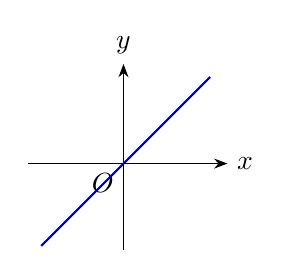
\begin{tikzpicture}[x=0.55cm,y=0.55cm,>=Stealth]
  \draw[->] (-2.2,0)--(2.4,0) node[right] {$x$};
  \draw[->] (0,-2.0)--(0,2.3) node[above] {$y$};
  \node[below left] at (0,0) {$O$};
  \draw[blue!70!black,thick] (-1.9,-1.9)--(2,2);
\end{tikzpicture}\par
\raggedright
定义域、值域均为 $\mathbb R$。\par
奇函数；在 $\mathbb R$ 上递增。
\end{column}
\begin{column}{0.48\textwidth}
\centering\textbf{$y=x^2$}\par
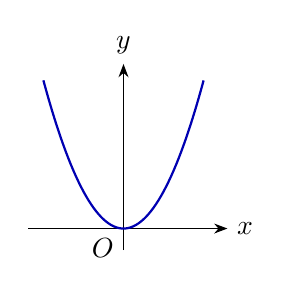
\begin{tikzpicture}[x=0.55cm,y=0.55cm,>=Stealth]
  \draw[->] (-2.2,0)--(2.4,0) node[right] {$x$};
  \draw[->] (0,-0.5)--(0,3.8) node[above] {$y$};
  \node[below left] at (0,0) {$O$};
  \draw[blue!70!black,thick,domain=-1.85:1.85,samples=65] plot (\x,{\x*\x});
\end{tikzpicture}\par
\raggedright
定义域 $\mathbb R$；值域 $[0,+\infty)$。\par
偶函数；在 $(-\infty,0]$ 上递减，\par
在 $[0,+\infty)$ 上递增。
\end{column}
\end{columns}
\Pitfall{$y=x^2$ 在整个 $\mathbb R$ 上没有同一种单调性。}
\end{frame}

\begin{frame}[t]{基本幂函数：立方函数与平方根函数}
\large
\Recall{哪个函数只允许非负输入？哪个函数的图象关于原点对称？}
\pause
\begin{columns}[T,onlytextwidth]
\begin{column}{0.48\textwidth}
\centering\textbf{$y=x^3$}\par
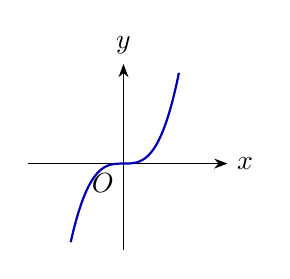
\begin{tikzpicture}[x=0.55cm,y=0.55cm,>=Stealth]
  \draw[->] (-2.2,0)--(2.4,0) node[right] {$x$};
  \draw[->] (0,-2.0)--(0,2.3) node[above] {$y$};
  \node[below left] at (0,0) {$O$};
  \draw[blue!70!black,thick,domain=-1.22:1.28,samples=65] plot (\x,{\x*\x*\x});
\end{tikzpicture}\par
\raggedright
定义域、值域均为 $\mathbb R$。\par
奇函数；在 $\mathbb R$ 上递增。
\end{column}
\begin{column}{0.48\textwidth}
\centering\textbf{$y=\sqrt{x}$}\par
\begin{tikzpicture}[x=0.55cm,y=0.55cm,>=Stealth]
  \draw[->] (-0.5,0)--(4.1,0) node[right] {$x$};
  \draw[->] (0,-0.5)--(0,3.8) node[above] {$y$};
  \node[below left] at (0,0) {$O$};
  \draw[blue!70!black,thick,domain=0:1.95,samples=65] plot ({\x*\x},\x);
\end{tikzpicture}\par
\raggedright
定义域、值域均为 $[0,+\infty)$。\par
非奇非偶；在 $[0,+\infty)$\par
上递增。
\end{column}
\end{columns}
\Pitfall{$\sqrt{x}$ 的定义域不关于原点对称；定义域和值域都包含 $0$。}
\end{frame}

\begin{frame}[t]{基本幂函数：$y=\dfrac1x$}
\large
\Recall{定义域、值域为什么排除 $0$？单调性要怎样分段表述？}
\pause
\begin{columns}[c,onlytextwidth]
\begin{column}{0.43\textwidth}
\centering
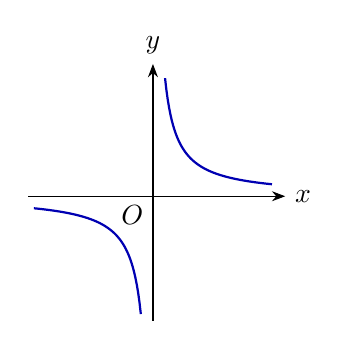
\begin{tikzpicture}[x=0.48cm,y=0.48cm,>=Stealth]
  \draw[->] (-3.3,0)--(3.5,0) node[right] {$x$};
  \draw[->] (0,-3.3)--(0,3.5) node[above] {$y$};
  \node[below left] at (0,0) {$O$};
  \draw[blue!70!black,thick,domain=0.32:3.15,samples=80] plot (\x,{1/\x});
  \draw[blue!70!black,thick,domain=-3.15:-0.32,samples=80] plot (\x,{1/\x});
\end{tikzpicture}
\end{column}
\begin{column}{0.54\textwidth}
\begin{itemize}
  \item 定义域：$\mathbb R\setminus\{0\}$。
  \item 值域：$\mathbb R\setminus\{0\}$。
  \item 奇函数；图象关于原点对称。
  \item 在 $(-\infty,0)$、$(0,+\infty)$\par\textbf{上分别递减}。
\end{itemize}
\end{column}
\end{columns}
\Pitfall{不能说它在整个定义域上递减；函数图象与两条坐标轴均无交点。}
\end{frame}


\begin{frame}[t]{第二节回忆：输入、输出与性质}
\Recall{遮住前面的知识，独立写出关键词，再回看补漏。}
\begin{enumerate}
\item 定义域、值域分别是什么？怎样检查解析式是否有意义？
\item 分段函数求值为什么先选段？
\item 单调性定义与证明怎样体现“任意”？
\item 判断奇偶性先检查什么，再比较什么？
\item 五个基本幂函数的图像与主要性质分别是什么？
\end{enumerate}
\pause
\par\vspace{0.2cm}\textbf{回看补漏：}区间范围、端点、任意性、定义域对称、分段表述。
\end{frame}

\Session{三}{根式、指数幂与指数函数}{根式与绝对值\quad 运算法则\quad 图像与性质}

% 第三节：根式、指数幂与指数函数。仅作知识回忆，不设例题。
\begin{frame}[t]{根与根式：奇次、偶次要分清}
\Recall{奇次根与偶次根有什么不同？偶次根式表示哪个根？}
\pause
\begin{itemize}
\item 若 $x^n=a$（$n\ge2$ 为整数），则 $x$ 是 $a$ 的 $n$ 次方根。
\item $n$ 为奇数：任意实数 $a$ 都有唯一的实数根，记作 $\sqrt[n]{a}$。
\item $n$ 为偶数：$a>0$ 有两个互为相反数的实数根；$a=0$ 只有根 $0$；$a<0$ 没有实数根。
\item 偶次根式 $\sqrt[n]{a}$ 表示\textbf{非负的根}，要求 $a\ge0$。
\end{itemize}
\Pitfall{“偶次方根”与“偶次算术根”要分清；根式前没有 $\pm$。}
\end{frame}

\begin{frame}[t]{开方与绝对值}
\Recall{先乘方再开方，结果一定等于原来的数吗？}
\pause
设 $n\ge2$ 为整数。对任意实数 $u$，有
\[
\sqrt[n]{u^n}=\begin{cases}u,&n\text{ 为奇数},\\ |u|,&n\text{ 为偶数}.\end{cases}
\]
\[
\boxed{\sqrt{u^2}=|u|}\qquad
|u|=\begin{cases}u,&u\ge0,\\-u,&u<0.\end{cases}
\]
\textbf{去绝对值的顺序：}先由条件判断内部式子的正负，再去绝对值。
\Pitfall{偶次根式的结果非负；不能直接把 $\sqrt{u^2}$ 写成 $u$。}
\end{frame}

\begin{frame}[t]{零指数与负指数}
\Recall{零指数幂的条件是什么？负指数表示什么？}
\pause
\begin{itemize}
\item 零指数：$\boxed{a^0=1\quad(a\ne0)}$。
\item 负指数：$\boxed{a^{-r}=\dfrac1{a^r}\quad(a>0,\ r>0)}$。
\item 若指数为整数，负底数也可运算，但底数必须非零。
\item $0$ 的正指数幂为 $0$；本课程中 $0^0$、$0$ 的负指数幂无意义。
\end{itemize}
\Pitfall{负指数表示取倒数；它不表示在结果前添负号。}
\end{frame}

\begin{frame}[t]{根式与分数指数幂互化}
\Recall{分数指数的分母、分子分别对应什么？}
\pause
\textbf{统一在 $a>0$ 下：}$m,n$ 为正整数，且 $n>1$。
\[
\boxed{a^{\frac mn}=\sqrt[n]{a^m}=(\sqrt[n]{a})^m}
\]
分母 $n$ 表示\textbf{开 $n$ 次方}，分子 $m$ 表示\textbf{乘 $m$ 次方}。
\[
a^{-\frac mn}=\frac1{a^{\frac mn}}=\frac1{\sqrt[n]{a^m}}.
\]
\Pitfall{先检查底数条件；带负号的分数指数还要取倒数。}
\end{frame}

\begin{frame}[t]{指数运算法则}
\Recall{同底相乘、相除、幂的乘方，指数分别怎样运算？}
\pause
\textbf{以下统一设 $a,b>0$，$r,s\in\mathbb R$：}
\[
\begin{aligned}
a^r\cdot a^s&=a^{r+s},&\qquad \frac{a^r}{a^s}&=a^{r-s},\\[0.35em]
(a^r)^s&=a^{rs},&(ab)^r&=a^rb^r,\\[0.35em]
\left(\frac ab\right)^r&=\frac{a^r}{b^r}.&&
\end{aligned}
\]
\Pitfall{相加没有“指数相加”的法则；$(a+b)^r$ 也不能按积的乘方法则拆开。}
\end{frame}

\begin{frame}[t]{根式与指数幂：整理顺序}
\Recall{面对含根号、负指数、小数和括号的式子，先检查什么？}
\pause
\begin{enumerate}
\item \textbf{看条件：}底数是否允许，分母是否为零，偶次根式是否有意义。
\item \textbf{先整理底数：}小数化分数，带分数化假分数，尽量化为幂。
\item \textbf{再整理指数：}根式与分数指数统一，负指数化为倒数。
\item \textbf{按顺序运算：}有括号先算括号内；先乘方，再乘除，最后加减。
\end{enumerate}
\Pitfall{负底数的整数次幂先看括号、再看奇偶；偶次根式化简别漏绝对值。}
\end{frame}

\begin{frame}[t]{指数函数的定义}
\Recall{指数函数中，谁是自变量？底数需要满足什么条件？}
\pause
\[
\boxed{y=a^x\qquad (a>0\text{ 且 }a\ne1)}
\]
\begin{itemize}
\item $a$ 是\textbf{固定的底数}，自变量 $x$ 在指数的位置。
\item 幂函数 $y=x^\alpha$ 中，自变量在底数的位置，指数 $\alpha$ 为常数。
\item 识别函数类型时，核对\textbf{完整形式}和\textbf{条件}。
\end{itemize}
\Pitfall{底数的两个条件都要写；$y=a^x$ 与 $y=x^a$ 的性质不同。}
\end{frame}

\begin{frame}[t]{指数函数的两类图像}
\Recall{底数大于 $1$ 与小于 $1$，图像各怎样变化？共同经过哪里？}
\pause
\begin{columns}[T,onlytextwidth]
\begin{column}{0.48\textwidth}\centering
$a>1$：从左向右上升\par
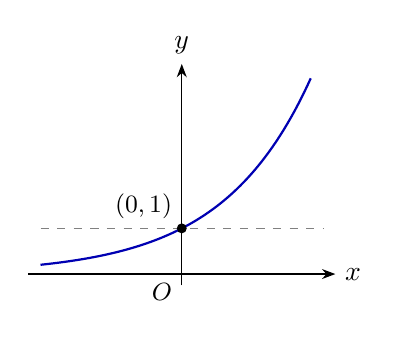
\begin{tikzpicture}[x=0.78cm,y=0.58cm,>=Stealth]
\draw[->](-2.5,0)--(2.5,0) node[right]{$x$};
\draw[->](0,-0.25)--(0,4.6) node[above]{$y$};
\draw[blue!70!black,thick,domain=-2.3:2.1,samples=70] plot(\x,{pow(2,\x)});
\draw[dashed,gray](-2.3,1)--(2.3,1);
\fill(0,1) circle(1.8pt) node[above left,font=\small]{$(0,1)$};
\node[below left,font=\small]at(0,0){$O$};
\end{tikzpicture}
\end{column}
\begin{column}{0.48\textwidth}\centering
$0<a<1$：从左向右下降\par
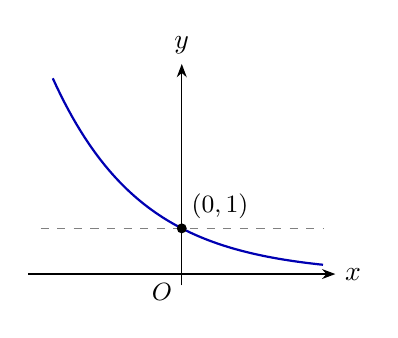
\begin{tikzpicture}[x=0.78cm,y=0.58cm,>=Stealth]
\draw[->](-2.5,0)--(2.5,0) node[right]{$x$};
\draw[->](0,-0.25)--(0,4.6) node[above]{$y$};
\draw[blue!70!black,thick,domain=-2.1:2.3,samples=70] plot(\x,{pow(2,-\x)});
\draw[dashed,gray](-2.3,1)--(2.3,1);
\fill(0,1) circle(1.8pt) node[above right,font=\small]{$(0,1)$};
\node[below left,font=\small]at(0,0){$O$};
\end{tikzpicture}
\end{column}
\end{columns}
\par\vspace{0.15cm}
共同性质：定义域 $\mathbb R$，值域 $(0,+\infty)$，图像过 $(0,1)$。
\Pitfall{图像始终在 $x$ 轴上方，函数值永远取不到 $0$。}
\end{frame}

\begin{frame}[t]{指数函数的单调性与比较大小}
\Recall{相同底数时，什么时候指数较大，函数值也较大？}
\pause
设 $u,v\in\mathbb R$，则
\[
\begin{array}{c|c|c}
\text{底数}&\text{单调性}&\text{比较规则}\\ \hline
a>1&\text{在 }\mathbb R\text{ 上递增}&a^u>a^v\ \Longleftrightarrow\ u>v\\[0.4em]
0<a<1&\text{在 }\mathbb R\text{ 上递减}&a^u>a^v\ \Longleftrightarrow\ u<v
\end{array}
\]
\textbf{比较步骤：}先看底数，尽量化为同底，再按单调性比较指数。
\Pitfall{“去掉同底幂”之前，必须判断底数在哪个范围。}
\end{frame}

\begin{frame}[t]{指数函数：范围与对称性}
\Recall{指数函数有没有最大值、最小值？两条互为倒数底数的曲线怎样对称？}
\pause
对 $y=a^x$（$a>0$ 且 $a\ne1$），在整个定义域 $\mathbb R$ 上：
\begin{itemize}
\item 值域为 $(0,+\infty)$，没有最大值，也没有最小值。
\item 是\textbf{非奇非偶函数}。
\item $y=a^x$ 与 $y=a^{-x}=\left(\dfrac1a\right)^x$ 的图像关于\textbf{$y$ 轴}对称。
\end{itemize}
\Pitfall{“互为倒数”是两式的关系；它不表示其中一条曲线关于 $y$ 轴对称。}
\end{frame}

\begin{frame}[t]{第三节回忆：指数幂与指数函数}
\Recall{先遮住知识内容，独立写出下列规则的完整形式与条件。}
\begin{enumerate}
\item 偶次根式化简时，绝对值出现在哪里？
\item 零指数、负指数、分数指数各怎样理解？
\item 同底乘除与幂的乘方，指数各怎样运算？
\item 指数函数的底数条件、定义域、值域、定点是什么？
\item 两类底数分别对应怎样的单调性？
\end{enumerate}
\pause
\par\vspace{0.2cm}\textbf{对照前页补漏：}条件、符号、括号、绝对值、增减方向。
\end{frame}


\begin{frame}[t]{最后十分钟：整理自己的遗漏}
\begin{enumerate}
\item 从今晚补写的内容中，选出自己仍记不牢的几条。
\item 每条写完整：\textbf{知识结论＋使用条件＋易错位置}。
\item 遮住完整内容，再独立写一遍，随后对照修正。
\end{enumerate}
\par\vspace{0.55cm}
\textbf{考试书写检查：}\par\vspace{0.25cm}
范围与端点\quad 不等号方向\quad 分母与根号\quad 等号与条件
\end{frame}
\end{document}
